% chktex-file 1
% chktex-file 13

\subsection{Distributed File Sharing}
\label{subsec:design-p2p}

\subsubsection*{Hash Tree}
\label{subsubsec:hash-tree}

The hash tree of a given directory is used to represent its structure as well as the contents of its files. Each file is represented by an ordered list of SHA-256 hashes that match a fixed-size block of data. This allows users to easily identify and verify game data \reqref{F-M10}.

\begin{figure}[ht]
  \centering
  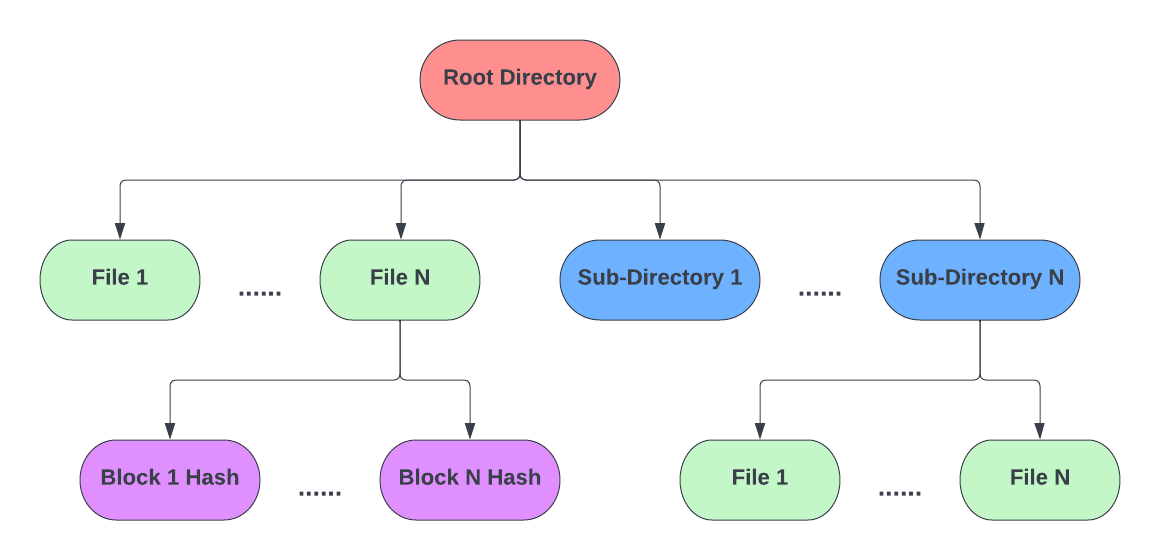
\includegraphics[width=.85\textwidth]{assets/images/diagrams/block-body.png}
  \caption{The structure of a hash tree}
  \label{fig:hash-storage}
\end{figure}

\subsubsection*{Uploading Content}
\label{subsubsec:upload-content}

For a developer to upload their game \reqref{F-M1}, they must provide the following:

\begin{itemize}
  \item the metadata outlined in Section~\ref{subsubsec:eth-data},
  \item a hash tree created from the root directory of the game, and
  \item an assets folder containing a piece of cover art \textit{(cover.png)} and a description file \textit{(description.md)}.
\end{itemize}

\vspace{2mm}\noindent
The developer should be able to enter the required fields into an upload page of the GUI and have the data generated and uploaded for them \reqref{F-S2}.

\subsubsection*{Downloading Content}

\newcommand{\seeder}{$P_{seeder}$~}
\newcommand{\downloader}{$P_{downloader}$~}

Like mentioned in Section~\ref{subsec:design-data}, it is impractical to store the game's data on the blockchain or IPFS. Instead we will consider ideas from decentralised file-sharing networks, like discussed in Sections~\ref{sec:lit-p2p} \&~\ref{sec:bittorrent}.
\x
Games are content addressable using their root hash field, which will allow users to request data from that game from other users. When a peer seeking data \downloader forms a connection with another peer \seeder they will:

\begin{enumerate}
  \item Perform a handshake to determine each other's Ethereum address and public key.
  \item \seeder will verify that \downloader owns the game by checking the \textit{purchased} mapping on the smart contract \reqref{F-M6} \reqref{F-S1}.
  \item \downloader will send requests for individual blocks to \seeder \reqref{F-M9}.
  \item Upon receiving a block, \downloader will verify the contents using the block's hash \reqref{F-M10} before writing it to disk in the appropriate location.
  \item Repeat Steps 3--4 until the entire game has been downloaded \reqref{F-M11}.
  \item \seeder may request a signed receipt that details the blocks they uploaded \reqref{F-S3} to \downloader.
\end{enumerate}

\vspace{2mm}\noindent
Users will be able to connect to many peers at once \reqref{F-M7} and will send download requests to the subset of their peers who also own the game. Requests will be sent in a round-robin fashion to evenly distribute the requests and prevent overloading a single peer \reqref{NF-S1}. Requests that cannot be completed will be retried when connecting to a new peer or when a peer has a change in library.

\subsubsection*{Updating Content}\label{subsubsec:updating}

To satisfy \reqref{F-M2}, developers will perform the same steps outlined in Section~\ref{subsubsec:upload-content} but must also provide the root hash of the most previous version of the game. Any users who have purchased the previous version will be added to the list of users who have purchased the new version \reqref{F-M3}. Additionally, this will include the restriction that only the original uploader can upload an update for their game \reqref{NF-M5}.
\x
Each version is considered its own game and will require users to download the updated version separately. Whilst this isn't reflective of how updates are typically managed, this will be acceptable for the scope of this project.

\subsubsection*{Downloadable Content}

Downloadable Content (DLC) \reqref{F-C1} represent optional additions for games that users will buy separately. DLCs will act similarly to how updates are treated. Each DLC will need:

\begin{enumerate}
  \item \textbf{Dependency} The root hash of the oldest version of the game this DLC supports.
  \item \textbf{Previous Version} (Optional) The root hash of the previous version of the DLC.
\end{enumerate}

\vspace{2mm}\noindent
Users must own the original game to buy any of its DLC. 

\subsubsection*{Proving Contribution}

As a user downloads blocks of data, they will keep track of which users have sent them which blocks. A peer may then request their contributions in the form of a signed message that can be sent to the developer \reqref{F-S3} in return for some kind of reward. The contents of the reward isn't specified for this project but could include in-game items, digital assets or Ether. This solution assumes that developers have knowledge of which Ethereum address maps to which of their game's users.